\section{Mersul lucrarii de laborator}

\subsection{Cerintele}

Initializarea unui nou repositoriu.\\
Configurarea VCS.\\
Commit, Push pe branch.\\
Folosirea fisierului .gitignore.\\
Revenire la versiunele anterioare.\\
Crearea branch-urilor noi.\\
Commit pe ambele branch-uri.\\
Merge la 2 branchuri.\\
Rezolvarea conflictelor.\\

\subsection{Analiza Lucrarii de laborator}
\tab Linkul la repozitoriu \textbf{https://github.com/Ernest96/MIDPS}\\
Sunt mai multe modalitati de a initializa un repozitoriu pe github.
Putem crea o mapa goala in care vom plasa gitul nostru prin intermediul comenzii \textbf{git init}.\\
\tab Urmatorul pas este crearea insusi a noului repozitoriu pe care il vom crea utilizind urmatoarea comanda
\textbf{curl -u 'USER' https.//api.github.com\\/user/repos -d '\{"name":"NUME"\}'}. Unde cuvintele scrise cu CAPS
se vor inlocui cu numele utilizatorului si numele repozitoriului.\\
\tab Dupa aceasta este necesar sa unim gitul nostru gol cu repozitoriul creat.
Vom folosi urmatoarea comanda \textbf{git remote add origin "Linkul la repo"}\\
\\
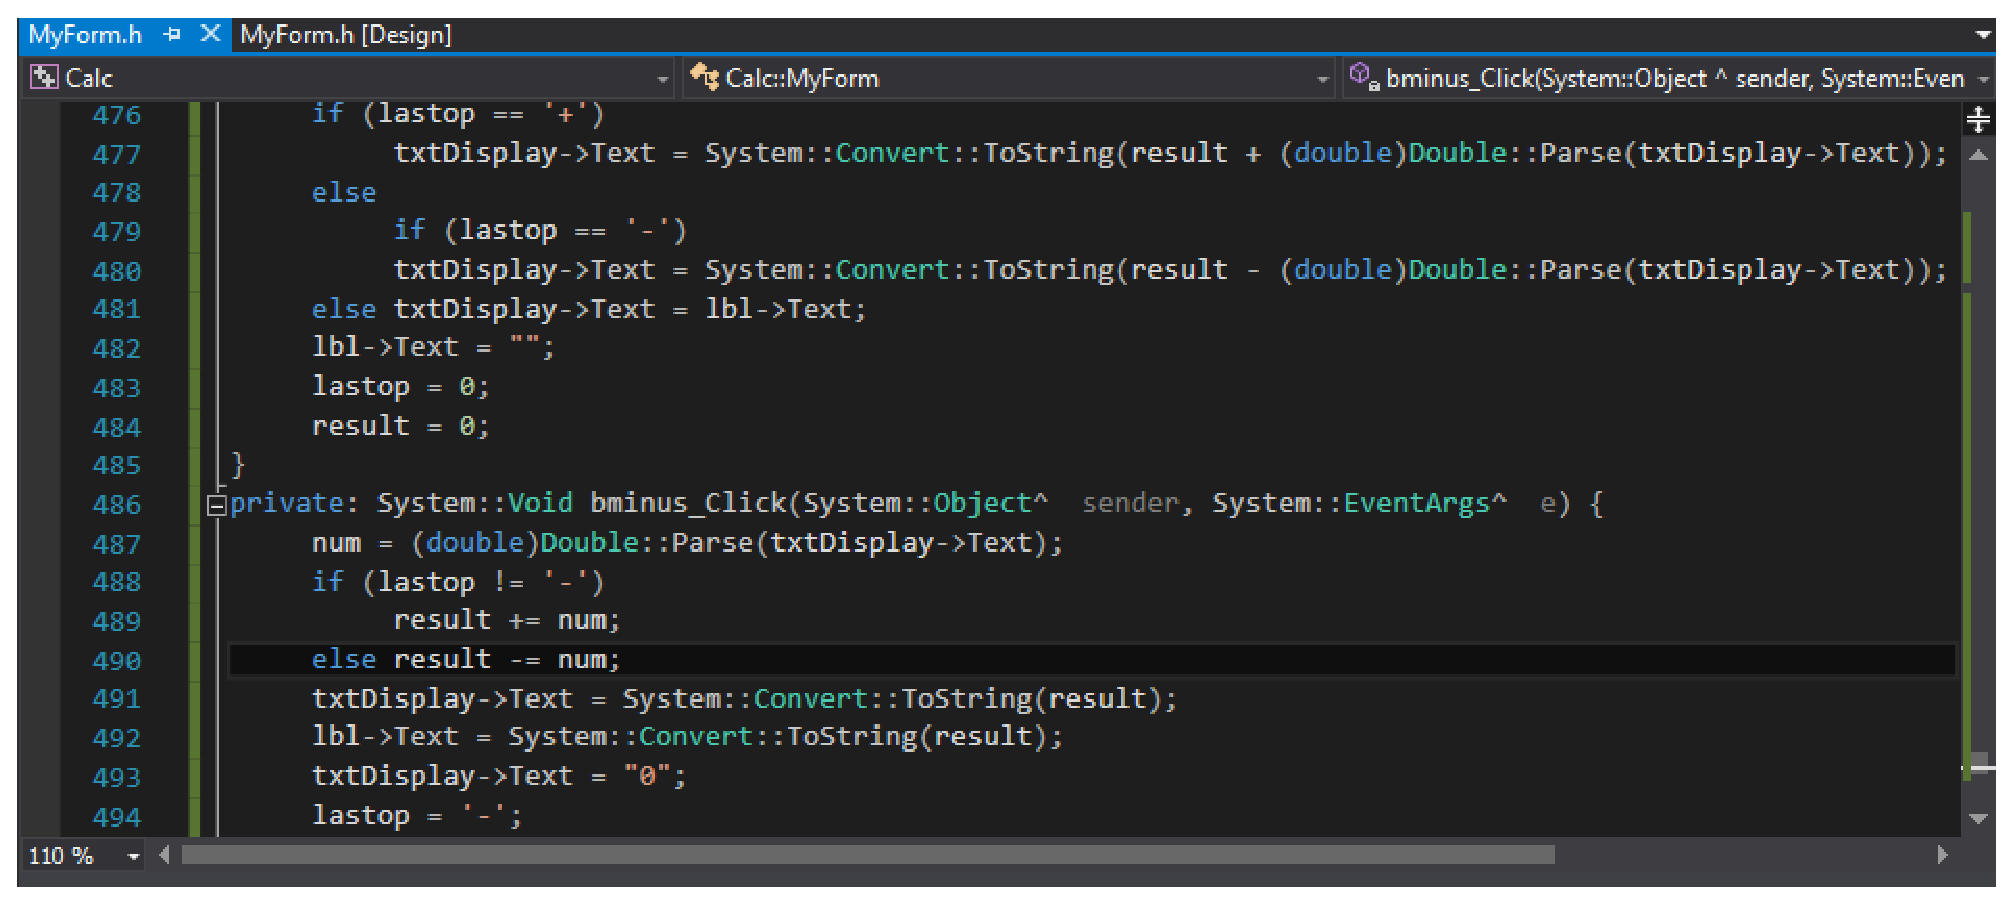
\includegraphics[width=\textwidth]{1.eps}
\clearpage
\tab O alta metoda de a crea un repozitoriu este cea online.
Pentru aceasta este nevoie sa deschidem pagina noastra pe github , sa alegem \textbf{repositories} si sa apasam butonul \textbf{new.}\\
\\
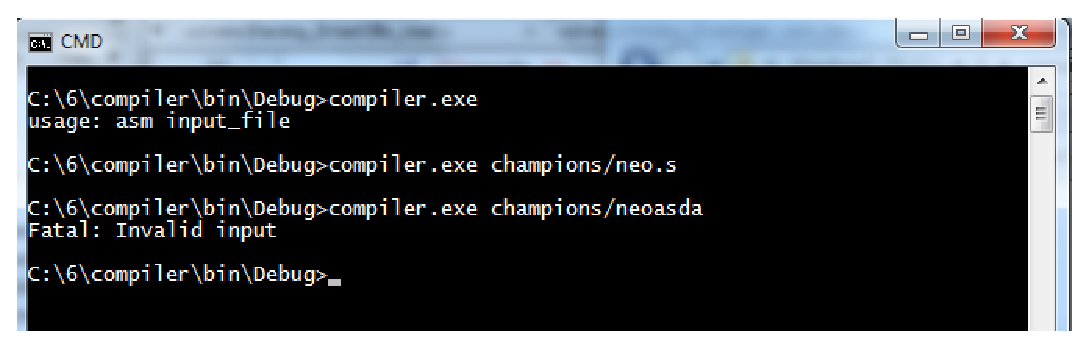
\includegraphics[width=\textwidth]{2.eps}
\\
\tab \textbf{Configurarea gitului} const in mai multe etape. La inceput vom configura numele si emailul.
Scrim urmatoarele comenzi:\\
\textbf{git config --global user.name "NUMELE"}\\
\textbf{git config --global user.email EMAIL}\\
\\
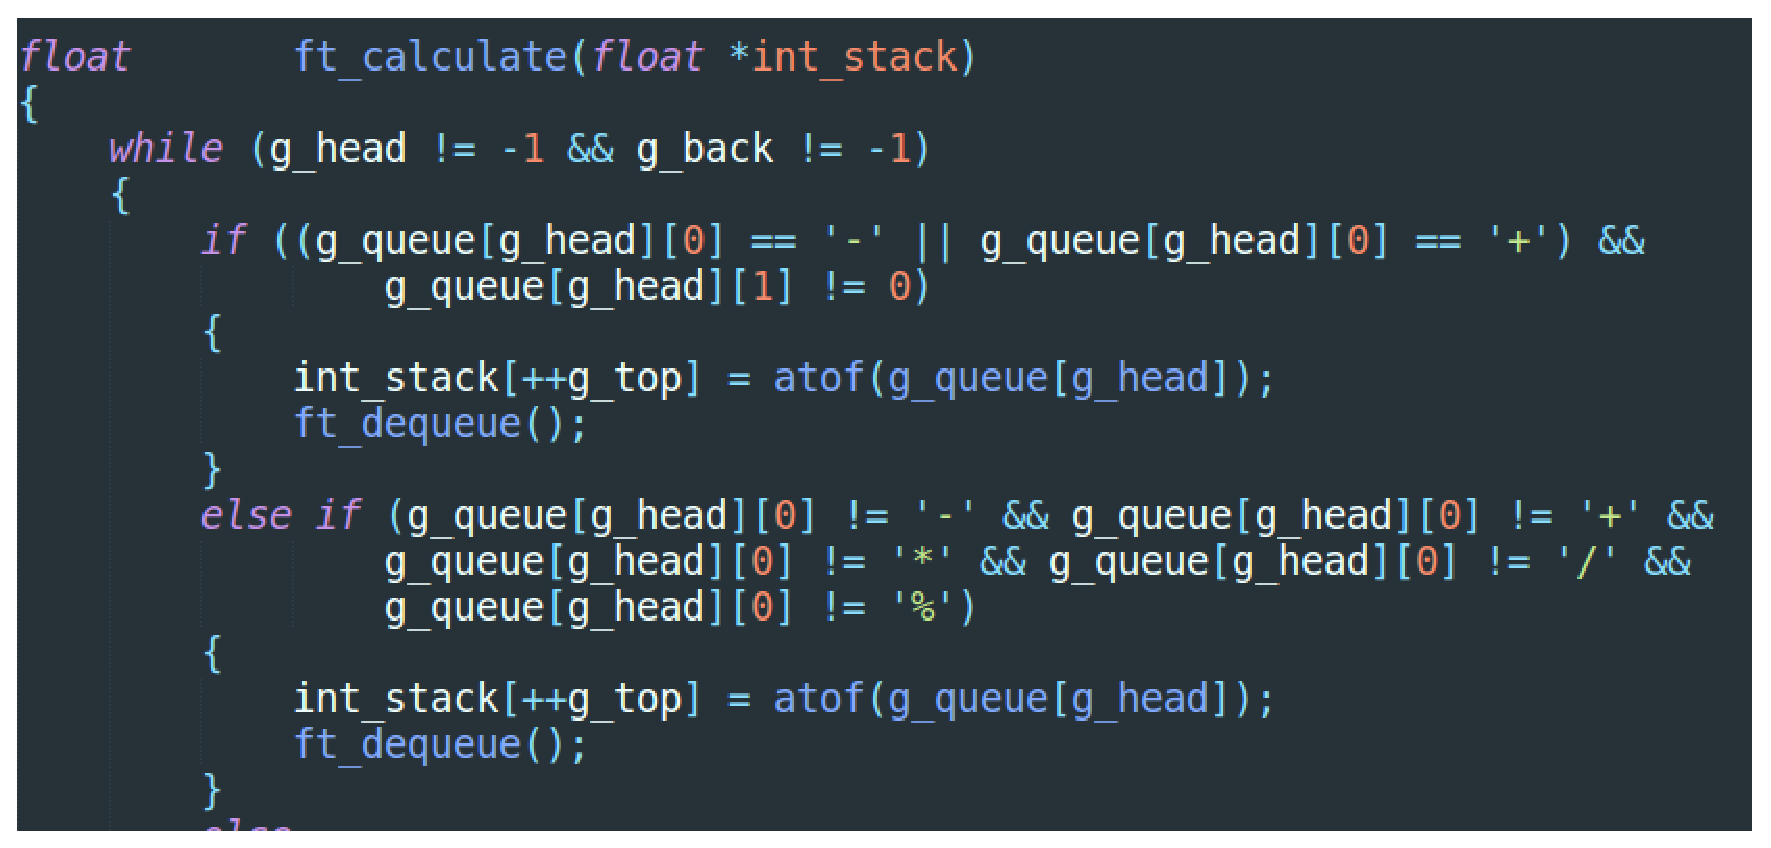
\includegraphics[width=\textwidth]{3.eps}
\\
\tab Urmatorul pas consta in generarea la cheia \textbf{SSH} (Secure Shell). Scriem in CLI \textbf{ssh-keygen},
iar cheia obtinuta o copiem in setarile noastre de pe git.
\tab Este de dorit sa initializam repozitoriul nostru cu un fisier \textbf{README.md} si un \textbf{.gitignore}. In fisierul
README.md vom adauga niste informatie pentru cei care se vor folosi de repozitoriu iar in fisierul .gitignore vom adauga
toate fisierele ce trebuiesc ignorate (adica sa nu fie incarcate).
\\
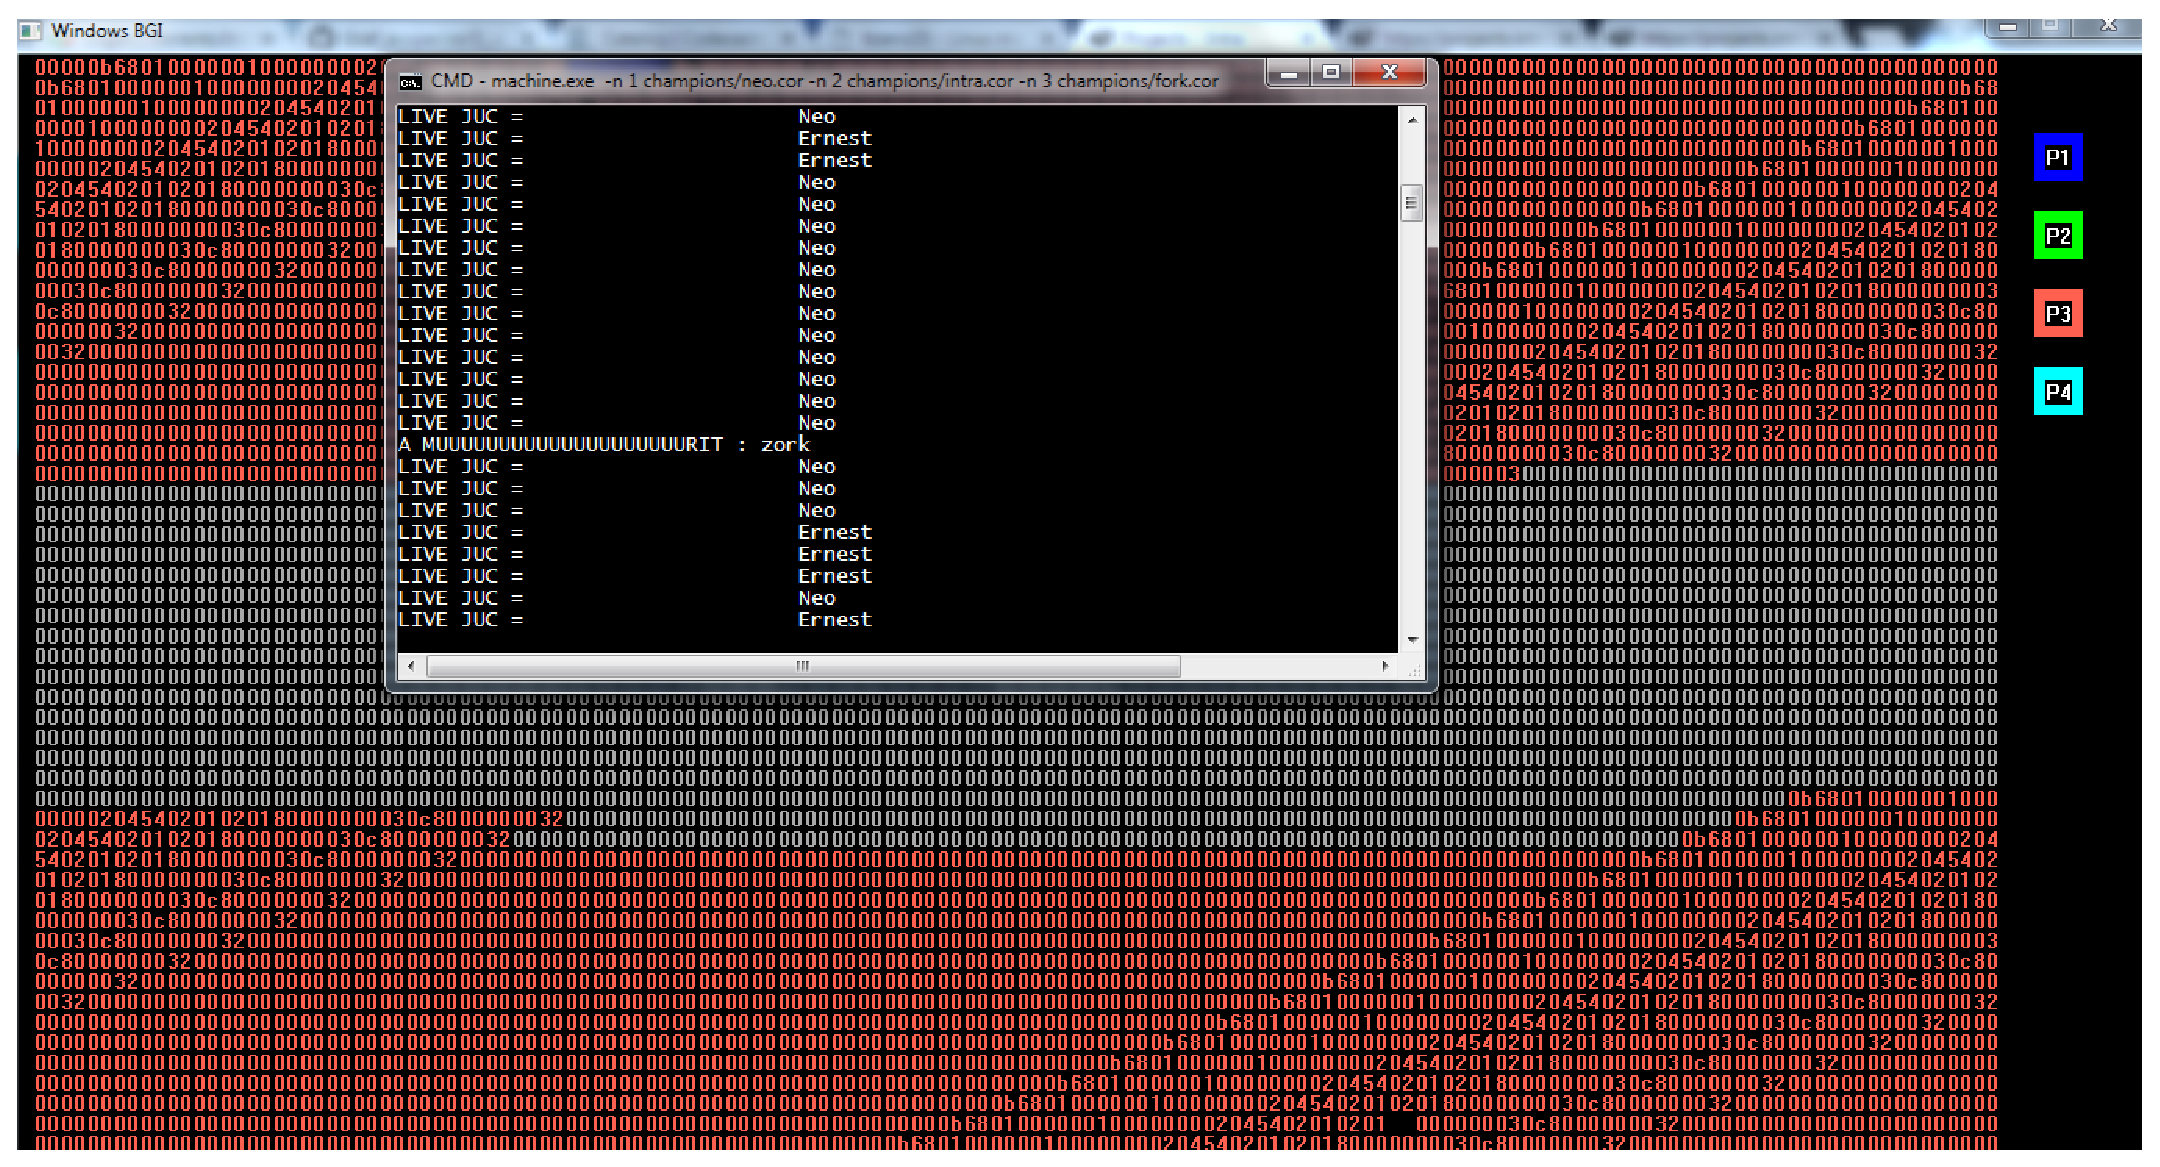
\includegraphics[width=\textwidth]{4.eps}
\\
\clearpage
